\documentclass[10pt,aps,prb,twocolumn, nofootinbib]{revtex4-1}

\usepackage{amssymb,amsmath}
\usepackage{subfig}
\usepackage{graphicx}
\usepackage{color}
\usepackage{hyperref}
\usepackage{listings}


\begin{document}

\title{Heat transport mechanisms for an end-heated aluminum rod}

\affiliation{Department of Nuclear Engineering, University of Wisconsin, Madison, WI, USA}
\date{\today}


\begin{abstract}
 Cover the motivation of the experiment, the general approach, as well as main results and/or conclusion.
\end{abstract}


\keywords{Keywords are listed below the abstract of the manuscript. At least three keywords are required at submission.}

\maketitle


\section{Introduction}
Include the motivation and purpose of the work and cover the relevant background information (e.g., physics and relevant formulas describing radiation-matter interactions).

\section{Approach}
Provide written description of the experiment and schematic of the setups.  Relevant experiment parameters and settings (e.g., discussion of how pressure is measured in the alpha-range lab and converted to effective distance between the source and detector, overall amplifier gains, applied voltages) should be included.

\section{Results}
Include relevant data and analyses, with brief descriptions of how they are derives.  Should include: 
\begin{itemize}
	\item Spectra illustrating the variation in energy/pulse height distribution of alpha particles at the detector as a function of chamber pressure.
	\item Plots of peak position and width (in channel number) as a function of chamber pressure.
	\item Plot of mean energy (E) as a function of effective distance (in cm or mg/cm$^{2}$)
	\item Plot of mean stopping power $\langle -\frac{dE}{dx} \rangle$ (in either MeV/cm or MeV/mg-cm$^{2}$) as a function of mean energy.
	\item Plot of detector count rate as a function of effective distance and calculation of th emean or extrapolated range.
	\item NaI scintillator spectra for the following conditions: Au-198 no absorber, Au-198 with Al absorber (at one thickness), Au-198 with Pb abasorber (at one thickness), and background.  Indicate on the spectrum the range of channels used to integrate counts in the photopeak.
	\item Plots of photopeak count rate as a function of AL absorber thickness (in g/cm$^2$), with and without background correction.
	\item Plots of photopeak count rate as a functio of Pb absorber thickness (in g/cm$^{2}$), with and without background correction.
	\item Fitted line and equation on the background-corrected gamma attenuated curve by the Al absorber, and calculation of the associated mass attenuation coefficient ((g/cm$^{2}$)$^{-1}$).
\end{itemize}

\begin{figure}[h!]
	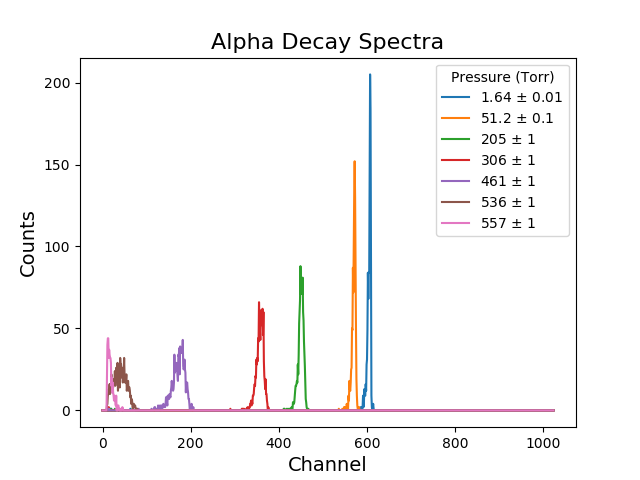
\includegraphics[width=.5\textwidth,keepaspectratio]{spectra_samples.png}
	\caption{Here we present a few sample spectra of the detected alpha particle decays at an assortment of pressures. \label{alph_spec}}
\end{figure} 

\begin{figure}[h!]
	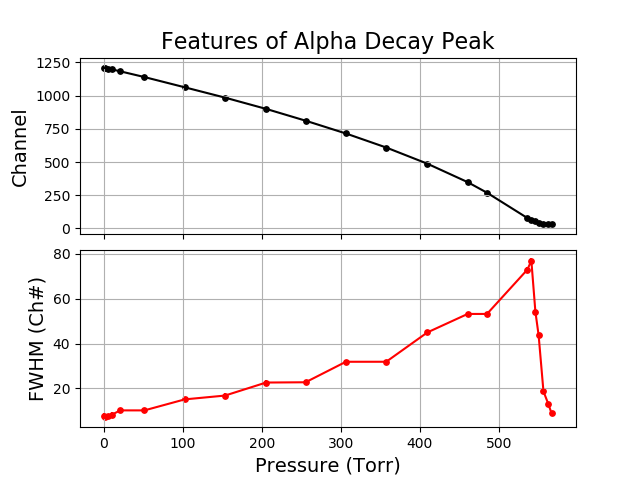
\includegraphics[width=.5\textwidth,keepaspectratio]{alf_peak_feat.png}
	\caption{Both of the above plots show particular features of the alpha decay peaks as a function of chamber pressure. (Top) is plotted the channel at which the alpha decay peak occurred, (Bottom) is plotted the FWHM in channel number of the alpha decay peak.  \label{alph_decay_feat}}
\end{figure} 

\begin{figure}[h!]
	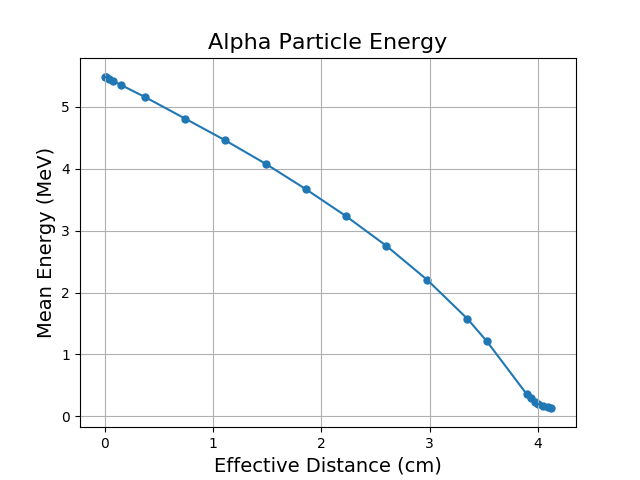
\includegraphics[width=.5\textwidth,keepaspectratio]{alph_energy.png}
	\caption{Here we present alpha particle energy as a function of the effective distance of the emitter source from the detector. \label{alph_energy}}
\end{figure} 

\begin{figure}[h!]
	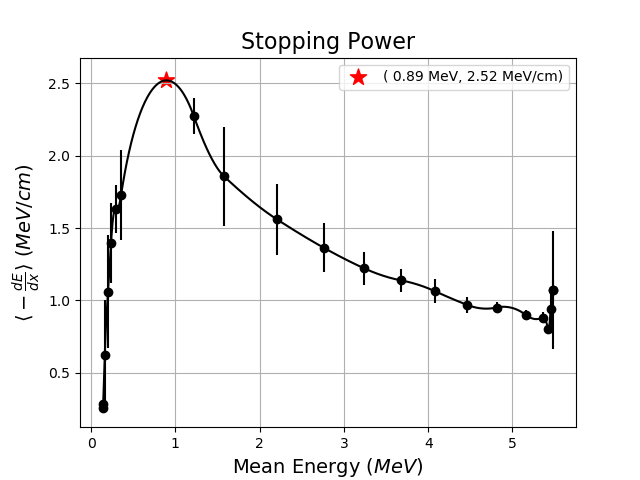
\includegraphics[width=.5\textwidth,keepaspectratio]{stop_pwr.png}
	\caption{Here we present the stopping power of the emitted alpha particles as a function of effective distance from the alpha emitter to the detector. \label{stop_pwr}}
\end{figure} 

\begin{figure}[h!]
	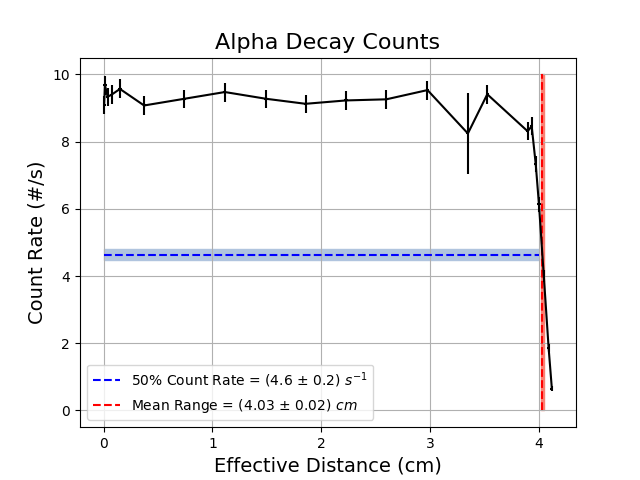
\includegraphics[width=.5\textwidth,keepaspectratio]{alf_peak_cnts.png}
	\caption{Here we present the alpha decay count rate as a function of the detector's effective distance from the source.  Included in the plot is our calculation of the mean range of the alpha particles (shown in red) as measured when the count rate drops to 50$\%$ its operational rate (shown in blue).  The shaded regions in the plot represent error in our measurements.   \label{alph_decay_cnts}}
\end{figure} 

\begin{figure*}[h!]
	\begin{tabular}{cccc}
		\subfloat[Background radiation spectra taken without a source. \label{gam_spec_back}]{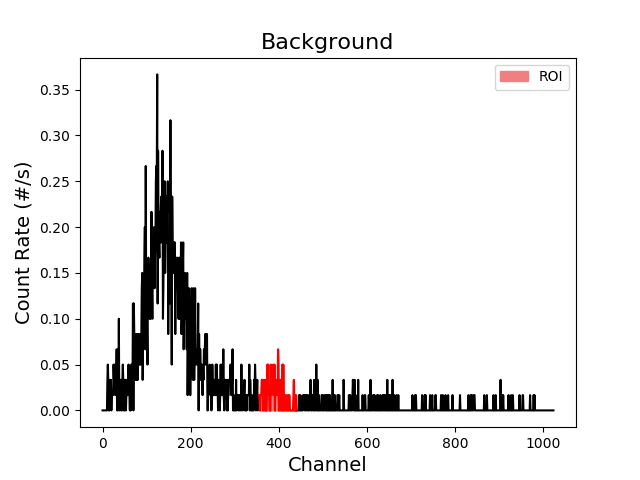
\includegraphics[width=.5\textwidth, keepaspectratio]{bckgrnd.png}} &
		\subfloat[Gamma decay spectra taken without a shield. \label{gam_spec_noShd}]{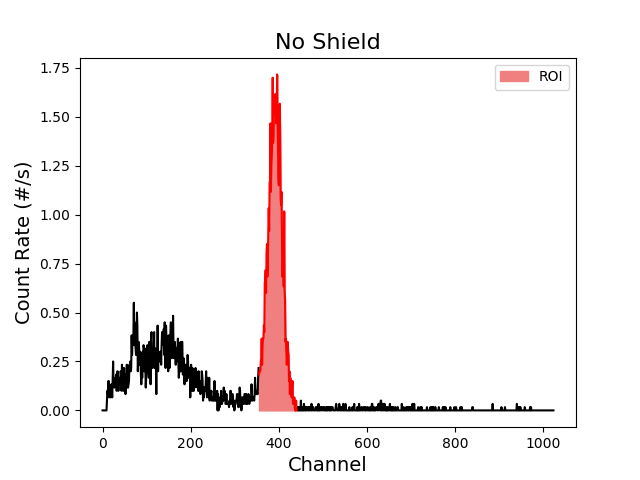
\includegraphics[width=.5\textwidth, keepaspectratio]{no_shield.png}} \\
		\subfloat[Gamma decay spectra with an Aluminum shield. \label{gam_spec_Al}]{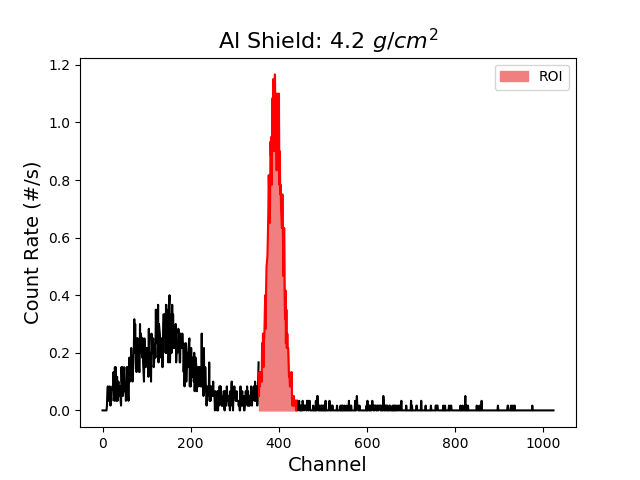
\includegraphics[width=.5\textwidth, keepaspectratio]{Al_shield.png}} &
		\subfloat[Gamma decay spectra with a Lead shield. \label{gam_spec_Pb}]{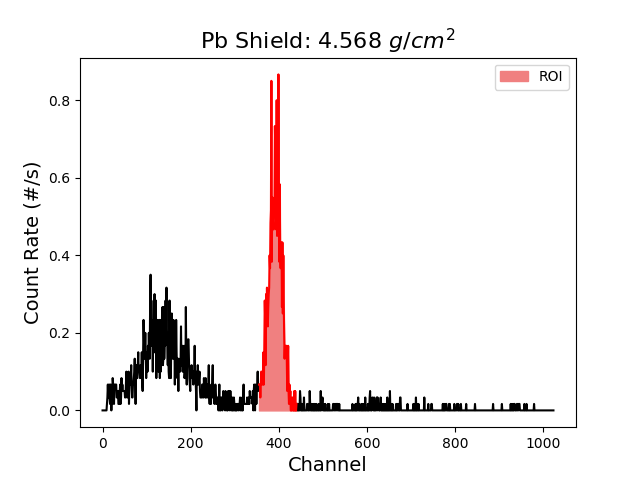
\includegraphics[width=.5\textwidth, keepaspectratio]{Pb_shield.png}}
	\end{tabular}
	\caption{Above are three spectra taken with a Au$^{198}$ gamma ray source and one spectra taken without any source. \label{gam_spec}}
\end{figure*}

\section{Discussion}
Includes explanations of the results and their significance.  Topics that should be addressed include (see "Analysisand discussion" section in lab manuel):

\begin{itemize}
	\item Change in peak shape and energy as a function of chamber pressure
	\item Dependence of mean stopping power on mean energy and effective distance.
	\item Comparison of th emean/extrapolated range obtained from your data with accepted values, and explanation of their difference.
	\item Explanation of why a collimated source is desired for the gamma attenuation measurement.
	\item Comparisons of the attenuation coefficients for Al and Pb obtained from your data with published values, and explanation of their difference.
	\item Description on how an alternative approach of measuring background data for the gamma attenuation experiments.
	\item Overall summary on your experiments
\end{itemize}


\begin{thebibliography}{99}
\bibitem{bib:1} C. Simenel, P. Chomaz, G. de France, Quantum calculation of dipole excitation in fusion reaction. Phys. Rev. Lett. {\bf 86}, 2971--2974 (2001). \href{http://dx.doi.org/10.1103/PhysRevLett.86.2971}{doi: 10.1103/PhysRevLett.86.2971}
\bibitem{bib:2} C. Tao, Y. G. Ma, G. Q. Zhang, \emph{et al}., Pygmy and giant dipole resonances by Coulomb excitation using a quantum molecular dynamics model. Phys. Rev. C, {\bf 87}: 014621 (2013). \href{http://dx.doi.org/10.1103/PhysRevC.87.014621}{DOI: 10.1103/PhysRevC.87.014621} 
\bibitem{bib:3} D.M. Abrams, in {\it Conductive Polymers}, ed. by R.S. Seymour, A. Smith (Springer, Berlin Heidelberg New York, 1973), p. 307 
\bibitem{bib:4} H. Ibach, H. Lüth, {\it Solid-State Physics}, 2nd edn. (Springer, New York, 1996), pp. 45–56 
\bibitem{bib:5} D. Zowghi et al., in {\it PRICAI '96: Topics in Artificial Intelligence}, ed. by N. Foo, R. Goebel. 4th Pacific Rim Conference on Artificial Intelligence, Cairns, August 1996. Lecture Notes in Computer Science. Lecture notes in artificial intelligence, vol. 1114 (Springer, Heidelberg, 1996), p. 157 
\end{thebibliography}



\end{document}